\documentclass[border=5mm]{standalone}
\usepackage{tikz}
\usetikzlibrary{cd}
\usetikzlibrary{decorations.pathmorphing,shapes,shapes.misc}
\begin{document}
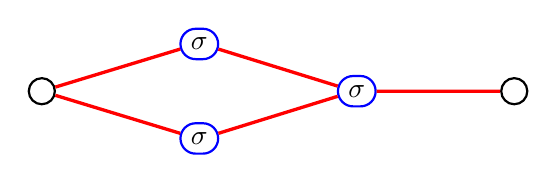
\begin{tikzpicture}
\begin{scope}[every node/.style={circle,thick,draw}]
    \node (A) at (0,0) {};
    \node (D) at (6,0) {};
\end{scope}
\begin{scope}[every node/.style={rounded rectangle,thick,draw=blue}]
    \node (B1) at (2,.6) {$\sigma$};
    \node (B2) at (2,-.6) {$\sigma$};
    \node (C) at (4,0) {$\sigma$};
\end{scope}
\begin{scope}[>={Stealth[black]},
              every edge/.style={draw=red,very thick}]
    \path [-] (A) edge node {}(B1.195);
    \path [-] (A) edge node {}(B2.165);
    \path [-] (B1.345) edge node {} (C.165);
    \path [-] (B2.15) edge node {} (C.195);
    \path [-] (C) edge node {} (D);
\end{scope}
\end{tikzpicture}
\end{document}  

%
%
%
%
%
%
%
%
%
%
%
%
%
%
%
%
%
%
%
%
%
%
%
%
%
%
%
%
















